\documentclass[10pt,wide]{mwart}
\usepackage{amsfonts}
\usepackage{amssymb}
\usepackage{graphicx}
\usepackage{svg}
\usepackage[utf8]{inputenc}
\usepackage{tikz}
\usepackage{tabularx}
%\usepackage{polski}
\usepackage[centertags]{amsmath}
\usepackage{amsthm}
\usepackage{newlfont}
\usepackage[polish]{babel}
\usepackage[T1]{fontenc}
\usepackage{listingsutf8}
\usepackage{xcolor}
\usepackage{url}
\newtheorem{lemat}{Lemat}
\newtheorem{tw}{Twierdzenie}
\newtheorem{przyklad}{Przykład}
\newtheorem{wn}{Wniosek}
\newtheorem{zad}{Zadanie}
\theoremstyle{definition}
\newtheorem{df}{Definicja}
\newtheorem{fc}{Fakt}
\newtheorem{uw}{Uwaga}
\newtheorem{szk}{Szkic dowodu}
\newtheorem{alg}{Algorytm}
\renewcommand*{\figurename}{Wykres}
\addto\captionspolish{\renewcommand{\figurename}{Wykres}}



%\textwidth 16cm
%\textheight 23.5cm
%\topmargin -1cm
%\oddsidemargin 0.5cm
%\evensidemargin 0.5cm
%\def\thefootnote{\arabic{footnote})}


\pagestyle{plain}
\begin{document}
\title{\textbf{Pracownia nr 3 z Analizy Numerycznej}\\
Sprawozdanie do zadania \textbf{P3.11}}
\author{Wiktor Garbarek}
\date{Wrocław, Styczeń 2018}

\maketitle
 \thispagestyle{empty}
\section{O całkach podwójnych i ich zastosowaniach praktycznych.}
Całki podwójne są dość intuicyjnym rozszerzeniem pojęcia całkowania funkcji jednej zmiennej.
Tak jak umiemy liczyć pole pod wykresem funkcji jednej zmiennej na określonym przedziale,
tak jednocześnie chcielibyśmy móc liczyć objętość pod wykresem funkcji dwóch zmiennych na określonym obszarze.
Jednak w przypadku analizy funkcji dwóch zmiennych i całek podwójnych pojawia się masa problemów.
W przypadku całek pojedynczych, obszarem całkowania naturalnie może być odcinek, czasami półprosta czy cała prosta, co nie sprawia aż tyle problemów.
Natomiast gdy rozpatrujemy całki podwójne, to nasz obszar całkowania może być zupełnie dowolny.
Od prostokąta, będącego po prostu iloczynem kartezjańskim dwóch przedziałów,
przez trójkąt czy koło, z którymi da się na jakieś sposoby poradzić,
kończąc na, w pewien sposób dowolnie zaznaczonych, fragmentach \(\mathbb{R}^2\) (nawet takich, które mają dziurki w środku!).

A ten problem jest dość ważny, chociażby dla trójwymiarowej grafiki komputerowej czy modelowania zjawisk fizycznych,
gdzie analiza funkcji dwóch zmiennych i umiejętność szybkiego i dokładnego policzenia całki na danym obszarze może rzutować
albo na wyglądzie sceny w grze lub filmie animowanym, czy na dokładności modelu fizycznego.


\section{Definicje używanych pojęć.}
Zaczniemy od rozszerzenia paru pojęć dotyczących wielomianów jednej zmiennej na wielomiany dwóch zmiennych.
\begin{df}
  Wielomianem dwóch zmiennych nazywamy funkcję
  \begin{equation}
    w(x,y) = \sum_{i=0}^{n} \sum_{j=0}^{m} a_{i,j}x^iy^j
  \end{equation}
\end{df}
\begin{df}(Stopień wielomianu dwóch zmiennych) \\
Jeśli \(w(x,y)\) ma postać (1), to
\begin{equation*}
  \deg(w) = max(\{i+j : a_{i,j} \neq 0\})
\end{equation*}
Ponadto przyjmiemy \(\deg_x(w) := \deg(w(x,1))\) oraz \(\deg_y := \deg(w(1,y))\), gdzie, jak łatwo zauważyć, wielomiany \(w(x,1)\) oraz \(w(1,y)\) są zwykłymi wielomianami jednej zmiennej.
\end{df}

Okazuje się jednak, że problem interpolacji w przypadku interpolacji wielomianem dwóch zmiennych jest nieco bardziej złożony.

\begin{tw}{Rozszerzenie postaci Lagrange'a wielomianu interpolacyjnego} \\
  Gdy interpolujemy funkcję \(f(x,y)\) w punktach \(P_i = (x_i,y_i)\) dla \( i = 0,...,n \), to
 \begin{equation*}
   L(x,y) = \sum_{i=0}^{n}\Big(f(x_i,y_i)\prod_{j = 0, j\neq i}^{n}\frac{(x-x_j)(y-y_j)}{(x_i - x_j)(y_i - y_j)}\Big)
 \end{equation*}
 jest wielomianem interpolacyjnym.
\end{tw}
\begin{uw}
  Gdy interpolujemy funkcję \(f(x,y)\) w punktach \((x_i, y_j)\) dla \( i = 0,...,n\) oraz \(j = 0,...,m\), to
  wygodniej będzie nam używać następującej postaci wynikającej wprost z powyższego wzoru
  \begin{equation*}
    L_{n,m}(x,y) = \sum_{i=0}^{n}\sum_{j=0}^m\Big(f(x_i,y_j)\prod_{k = 0, k\neq i}^{n}\frac{x-x_k}{x_i - x_k} \prod_{l=0, l \neq j}^{m}\frac{y-y_l}{y_j - y_l}\Big)
  \end{equation*}
\end{uw}

\begin{tw}
  Wielomian inteprolacyjny stopnia \(\leq n\) jest ustalony jednoznacznie dla \(\frac{(n+1)(n+2)}{2}\) punktów.
\end{tw}
Intuicyjnie możemy to postrzegać w ten sposób, że gdy dodawaliśmy kolejny punkt w przypadku interpolacji funkcji \(f(x)\) to rozszerzaliśmy o jeden wielomian bazę \(\Pi_n\) przez wielomian \(x^{n+1}\)
- natomiast w przypadku dwuwymiarowym interpolując funkcję \(f(x,y)\) bazę \(\Pi_n^2\) rozszerzamy bazę o dokładnie \(n+2\) wielomianów, a dokładniej przez zbiór \(\{x^{n+1}, x^{n}y, x^{n-1}y^2, ... y^{n+1}\}\).
W takim razie minimalna potrzebna ilość punktów by wyrazić wielomian stopnia n jest równa \(1 + 2 + 3 + 4 ... + n + (n+1) = \frac{(n+1)(n+2)}{2}\).
Ogólniej, w przypadku wielowymiarowym, by funkcję k-zmiennych f zinterpolować w sposób jednoznaczny przez wielomian k-zmiennych, to potrzebujemy dokładnie \({n+k \choose k}\) punktów,
 a szczegółowy dowód możemy zobaczyć w \cite{PO}.
\begin{tw} (Błąd interpolacji funkcji dwóch zmiennych)
  Niech \(L_{n,m}(x,y)\) interpoluje funkcję \(f(x,y)\) w \((n+1)(m+1)\) punktach postaci \((x_i, y_j)\) dla \(i = 0,...,n\) oraz \(j = 0,...,m\)
  Wtedy istnieją takie \( a \leq \xi,\xi' \leq b\) oraz \(c \leq \eta,\eta' \leq d\), że
  \begin{equation*}
    \begin{split}
  f(x,y) - L_{n,m}(x,y) & = \frac{1}{(n+1)!}\frac{\partial^{n+1} f(\xi, y)}{\partial x^{n+1}}w_{n+1}^{(x)}(x) + \frac{1}{(m+1)!}\frac{\partial^{m+1} f(x, \eta)}{\partial y^{m+1}}w_{n+1}^{(y)}(y)\\
  & - \frac{1}{(n+1)!(m+1)!}\frac{\partial^{n+1 + m+1} f(\xi',\eta') }{\partial x^{n+1} \partial y^{m+1}}w_{n+1}^{(x)}(x)w_{m+1}^{(y)}(y)
  \end{split}
\end{equation*}
gdzie \(w_{n+1}^{(x)}(x) = \prod_{i=0}^{n}(x-x_i)\) oraz \(w_{n+1}^{(y)}(y) = \prod_{j=0}^{m}(y-y_j)\).
\end{tw}
Wzór ten możemy wyprowadzić wykorzystując kilkukrotnie wzór na resztę interpolacji funkcji jednej zmiennej. Szczegółowy dowód tego twierdzenia można odnaleźć w \cite[\S6.6]{IK}.
\begin{df}(Rząd kubatury) \\
  Przedstawimy definicję analogiczną do rzędu kwadratur funkcji jednej zmiennej.
  Niech \(\Pi_{n}^2\) będzie zbiorem wszystkich wielomianów dwóch zmiennych stopnia co najwyżej \(n\), a \(R_n^C\) jest funkcją reszty kubatury \(C_n\) tj.
  \begin{equation*}
    |R_n^C| = \Big|\int_a^b \int_c^d f(x,y) p(x,y) dx dy - C_n(f)\Big|
  \end{equation*}
  Będziemy mówić, że kubatura \(C_n\) jest rzędu \(r\) jeśli
  dla dowolnego wielomianu dwóch zmiennych \(w \in \Pi_{r-1}^2\) zachodzi \(R_n^C(w) = 0 \)
  oraz istnieje wielomian \(w \in \Pi_{r}^2 \setminus \Pi_{r-1}^2\) taki, że \(R_n^C(w) \neq 0\)


\end{df}

\section{Kubatury Newtona-Cotesa.}
\subsection{Rozszerzenie kwadratur Newtona-Cotesa.}
W przypadku całki pojedynczej, interpretacja graficzna wzoru trapezów była bardzo prosta - szukaną całką było pole trapezu. Takiej samej interpretacji nie możemy wykorzystać jednak we wzorze trapezów dla całek podwójnych.
 Powód jest prosty: jeśli będziemy całkować w rogach naszego obszaru, to mamy 4 punkty, a każda płaszczyzna jest wyznaczona jednoznacznie przez 3 punkty. Jednakże mamy pewną przewagę nad interpretacją graficzną -
 wiemy, że wzór trapezów (tak jak zresztą inne kwadratury Newtona-Cotesa) pochodziły wprost z wielomianu interpolacyjnego dla funkcji f (dla wzoru trapezów mieliśmy interpolację w dwóch punktach).
 Wykorzystamy tą interpretację dla całek podwójnych.

\begin{tw} (Współczynniki kubatur Newtona-Cotesa.) \\
  Dana jest funkcja \(f: \mathbb{R}^2 \rightarrow \mathbb{R}\).
  Niech \(  L_{n,m}(x,y) = \sum_{i=0}^{n}\sum_{j=0}^m\Big(f(x_i,y_j)\prod_{k = 0, k\neq i}^{n}\frac{x-x_k}{x_i - x_k} \prod_{l=0, l \neq j}^{m}\frac{y-y_l}{y_j - y_l}\Big)\)
  będzie wielomianem interpolacyjnym funkcji f.
  Wtedy
  \begin{equation*}
    \int_a^b \int_c^d f(x,y) dy dx \approx C_{n,m}^{NC}(f) = \sum_{i=0}^{n}\sum_{j=0}^{n}W_{i,j}f(x_i,y_j)
  \end{equation*}
  a \(W_{i,j} := A_i^{(n)}A_j^{(m)}\), gdzie \(A_k^{(n)}\) to k-ty współczynnik n-tej kwadratury Newtona-Cotesa dla funkcji jednej zmiennej.
    \begin{proof}
    Łatwo widzieć jak wygląda waga \(W_{i,j}\) na podstawie postaci wyrażenia \(L_{n,m}\).
  \begin{equation*}
    \begin{split}
  W_{i,j} & = \int_a^b \int_c^d \prod_{k = 0, k\neq i}^{n}\frac{x-x_k}{x_i - x_k} \prod_{l=0, l \neq j}^{n}\frac{y-y_l}{y_j - y_l} dydx \\
  & = \int_a^b \int_c^d \lambda_i(x)\lambda_j(y) dy dx \\
  & = \Big(\int_a^b \lambda_i(x) dx\Big)\Big(\int_c^d \lambda_j(y)dy\Big) \\
  & = A_i^{(n)}A_j^{(m)}
    \end{split}
  \end{equation*}
\end{proof}
\end{tw}
Oszacujmy także rząd kubatur Newtona-Cotesa, wykorzystuąc wzór na resztę wielomianu interpolacyjnego (Twierdzenie 3).
Z jednej strony możemy zauważyć, że na pewno wszystkie wielomiany interpolacyjne funkcji będących wielomianami stopnia co najwyżej \(min(m,n)\) zostaną policzone dokładnie.
Z drugiej strony, możemy zauważyć, że skoro twierdzenie o błędzie interpolacji wynikało z zastosowania twierdzenia o błędzie interpolacji funkcji jednej zmiennej, to w takim razie, analogicznie do błędów kwadratur Newtona-Cotesa dowiemy się, że
to możemy przewidywać, że rząd kubatur Newtona-Cotesa jest równy \(r = \min(m,n)+1\) gdy \(\min(m,n)\) jest nieparzyste, a \(r = \min(m,n) + 2\) gdy \(\min(n,m)\) jest parzyste.
 \subsubsection{Wzór Trapezów}
 Gdy liczymy całkę \(\int_a^b \int_c^d f(x,y) dy dx\), to najpierw chcemy interpolować \(f(x,y)\) w czterech punktach - mianowicie w (a,c),(a,d),(b,c),(b,d).

 \begin{equation*}
   f(x,y) \approx \frac{(x-b)(y-d)}{(a-b)(c-d)}f(a,c) + \frac{(x-b)(y-c)}{(a-b)(d-c)}f(a,d) + \frac{(x-a)(y-d)}{(b-a)(c-d)}f(b,c) + \frac{(x-a)(y-c)}{(b-a)(d-c)}f(b,d)
 \end{equation*}
Zgodnie z udowodnionym twierdzeniem o współczynnikach kubatur Newtona-Cotesa, nasze współczynniki \(W_{i,j} = A^{1}_iA^{1}_j \equiv \frac{1}{2\cdot2} = \frac{1}{4}\)
Nasz wzór trapezów przybiera postać
\begin{equation}
\int_a^b \int_c^d f(x,y) dy dx \approx C_{1,1}^{NC}(f) = \frac{(b-a)(d-c)}{4}\Big(w(a,c) + w(a,d) + w(b,c) + w(b,d)\Big)
\end{equation}
\subsubsection{Wzór Simpsona}
Znowu chcemy wykorzystać interpolację - tym razem w 9 punktach postaci \((x_i, y_j)\) gdzie \(x_i = a + i*(b-a)/2\) dla \(i = 0,1,2\) oraz \(y_j = c + j*(d-c)/2\) dla \(j = 0,1,2\).
\begin{equation*}
  f(x,y) \approx  \sum_{i=0}^{2}\sum_{j=0}^2\Big(f(x_i,y_j)\prod_{k = 0, k\neq i}^{2}\frac{x-x_k}{x_i - x_k} \prod_{l=0, l \neq j}^{2}\frac{y-y_l}{y_j - y_l}\Big)
\end{equation*}
Analogicznie jak w przypadku wzoru trapezów otrzymujemy
\begin{equation}
  \begin{split}
  \int_a^b \int_c^d f(x,y) dy dx \approx C_{2,2}^{NC}(f) = \frac{(b-a)(d-c)}{9}(& f(a,c) + 4f(\frac{a+b}{2}, c) + f(b,c) + \\
                                                              &+ 4f(a, \frac{c+d}{2})+16f(\frac{a+b}{2}, \frac{c+d}{2}) + 4f(b, \frac{c+d}{2}) + \\
                                                              & + f(a,d) + 4f(\frac{a+b}{2},d) + f(b,d))
\end{split}
\end{equation}
\subsubsection{Przypadek ogólny.}
Kubatury Newtona-Cotesa bardzo łatwo się rozszerzają do przypadku dwuwymiarowego, gdy całkujemy po prostokącie, szczególnie za sprawą twierdzenia o współczynnikach kubatur Newtona-Cotesa, które przedstawiliśmy wcześniej.
Możemy też wysnuć hipotezę, że gdy rozważamy całkę z funkcji n-zmiennych, gdy obszarem całkowania są odpowiedniki prostokątów (czyli prostopadłościany czy hiperprostopadłościany wielowymiarowe) to współczynniki kubatury są po prostu odpowiednimi iloczynami współczynników dla przypadku jednowymiarowego.
Wartym zauważenia też jest fakt, że metoda ta nie koniecznie musi oznaczać całkowanie po prostokącie - z łatwością możemy zauważyć, że dość popularne całkowanie w układzie biegunowym wyznacza koło (bądź jego wycinek) w układzie Kartezjańskim, ale jest to pewien odpowiednik prostokąta w układzie biegunowym.

Jak dobrze pamiętamy, w przypadku jednowymiarowym interpolacja w węzłach równoodległych dla funkcji \(f(x) = \frac{1}{1+x^2}\) powodowała efekt Rungego,
a co za tym idzie wpływała na dokładność wyniku kwadratur Newtona-Cotesa. Okazuje się, że podobny efekt zachodzi dla funkcji \(f(x,y) = \frac{1}{1+25x^2 + 25y^2} \).


\subsection{Złożone kubatury Newtona-Cotesa.}
Analogicznie jak w przypadku jednowymiarowym mogliśmy podzielić sobie przedział całkowania na \(n\) równej długości podprzedziałów,
tak samo tutaj prostokąt \([a,b]\times [c,d]\) możemy podzielić sobie na \(n\cdot m\) mniejszych prostokątów.
W każdym mniejszym prostokącie przybliżamy całkę za pomocą kubatury trapezów, albo kubatury Simpsona.
W takim razie dla złożonej kubatury trapezów otrzymujemy wzór
\begin{equation}
  C^T_{m,n} = \frac{(b-a)(d-c)}{4mn}\sum_{i=0}^{n}\sum_{j=0}^{m}W_{i,j}f(x_i,y_j)
\end{equation}
gdzie wagi W są następującą macierzą
\begin{equation*}
  W =
\begin{bmatrix}
    1 & 2 & 2 & \dots  & 2 & 2 & 1 \\
    2 & 4 & 4 & \dots  & 4 & 4 & 1 \\
    2 & 4 & 4 & \dots  & 4 & 4 & 1 \\
    2 & 4 & 4 & \dots  & 4 & 4 & 1 \\
    \vdots & \vdots & \vdots & \ddots & \vdots & \vdots & \vdots \\
    2 & 4 & 4 & \dots  & 4 & 4 & 1 \\
    1 & 2 & 2 & \dots  & 2 & 2 & 1 \\
\end{bmatrix}
\end{equation*}
Dla złożonej kubatury Simpsona otrzymujemy wzór
\begin{equation}
  C^S_{m,n} = \frac{(b-a)(d-c)}{9mn}\sum_{i=0}^{n}\sum_{j=0}^{m}W_{i,j}f(x_i,y_j)
\end{equation}
gdzie wagi W są następującą macierzą
\begin{equation*}
  W =
\begin{bmatrix}
    1 & 4 & 2 & 4 & 2 &\dots  & 2 & 4 & 1 \\
    4 & 16 & 8 & 16 & 8 &\dots  & 8 & 16 & 1 \\
    2 & 8 & 4 & 8 & 4 &\dots  & 4 & 8 & 1 \\
    4 & 16 & 8 & 16 & 8 &\dots  & 8 & 16 & 1 \\
    \vdots & \vdots & \vdots & \vdots & \vdots &\ddots & \vdots & \vdots & \vdots \\
    4 & 16 & 8 & 16 & 8 &\dots  & 8 & 16 & 1 \\
    1 & 4 & 2 & 4 & 2 &\dots  & 2 & 4 & 1 \\
\end{bmatrix}
\end{equation*}

\section{Kubatury Gaussa.}
\subsection{Wagi postaci \(w(x,y) = w_1(x)w_2(y)\).}
Zacznijmy od następującego twierdzenia.
\begin{tw}
  Niech \(w(x,y) = w_1(x)w_2(y)\) \\
  Bazą ortogonalną dla iloczynu skalarnego \(\langle f,g \rangle = \int_a^b\int_c^d f(x,y)g(x,y)w(x,y)dydx\) jest ciąg wielomianów
  \begin{equation*}
    P_k^n(x,y) = p_k(x)q_{n-k}(y)
  \end{equation*} gdzie \(p_k\) jest ciągiem wielomianów ortogonalnych dla \(\langle f,g \rangle = \int_a^b f(x)g(x)w_1(x) dx\),
  a \(q_k\) jest ciągiem wielomianów ortogonalnych dla \(\langle f,g \rangle = \int_c^d f(x)g(x)w_2(x)dx\)
\end{tw}
Szczegółowy dowód tego twierdzenia możemy znaleźć w \cite{PS} oraz w \cite{YX}.
Dzięki temu, możemy łatwo zauważyć, że dowolną kwadraturę Gaussa (bądź dowolne pary kwadratur Gaussa) możemy rozszerzyć na przypadek dwuwymiarowy, w sposób analogiczny do metod Newtona-Cotesa.
\begin{tw} (Współczynniki kubatur Gaussa)
  Gdy \(w(x,y) = w_1(x)w_2(y)\)
  Możemy popatrzeć na nie jako kubaturę interpolacyjną w zerach wielomianu \(P_k^n(x,y) = p_k(x)q_{n-k}(y)\). Mamy wielomian interpolacyjny interpolujący po parach punktów \(\Big\{(x,y) : p_k(x) = 0 \wedge q_{n-k}(y) = 0\Big\} = ker(p_k) \times ker(q_{n-k})\)
  Niech więc ciąg \(x_1, x_2, ..., x_k\) będzie ciągiem zer funkcji \(p_k(x)\), a ciąg \(y_1, y_2, ..., y_{n-k}\) - ciągiem zer funkcji \(q_{n-k}(y)\).
  Zgodnie z założeniami, wielomian interpolacyjny wygląda następująco
  \begin{equation*}
    L_{n,k}(x,y) = \sum_{i=1}^{k}\sum_{j=1}^{n-k}\Big(f(x_i,y_j)\prod_{l = 1, l\neq i}^{k}\frac{x-x_l}{x_i - x_l} \prod_{m=1, m \neq j}^{n-k}\frac{y-y_m}{y_j - y_m}\Big)
  \end{equation*}
  Łatwo zauważyć, że nasza kubatura przybiera następującą postać
  \begin{equation*}
    C_{n,k}(f) = \sum_{i=1}^k\sum_{j=1}^{n-k}W_{i,j}f(x_i,y_j)
  \end{equation*}
  \begin{equation*}
  \begin{split}
    W_{i,j} & = \int_a^b \int_c^d \Big(\prod_{l = 1, l\neq i}^{k}\frac{x-x_l}{x_i - x_l} \prod_{m=1, m \neq j}^{n-k}\frac{y-y_m}{y_j - y_m}\Big) w(x,y)dy dx \\
    & = \int_a^b \int_c^d \lambda_k^{(p)}(x) \lambda_j^{(q)}(y) w_1(x)w_2(y) dydx \\
    & = \Big(\int_a^b \lambda_k^{(p)}(x) w_1(x) dx\Big)\Big( \int_c^d \lambda_j^{(q)}(y) w_2(y) dy\Big) \\
    & = A_i^{(k)}\cdot B_j^{(n-k)}
  \end{split}
\end{equation*}
  Gdzie \(A_i^{(k)}\) jest i-tym współczynnikiem jednowymiarowej kwadratury Gaussa dla ciągu wielomianów \(p_k\), a \(B_j^{(n-k)}\) - j-tym dla kwadratury dla ciągu wielomianów \(q_{n-k}\)
\end{tw}
Warto zauważyć, że możemy w dowolny sposób dobrać pary ciągów wielomianów ortogonalnych, by otrzymać kubaturę.

\subsubsection{Podwójna kubatura Gaussa-Czebyszewa.}
Omówimy przykład kubatury w zerach wielomianu \(T_n^{n+m}(x,y) = T_n(x)T_m(y)\).
Wiemy, że w przypadku jednowymiarowym mamy kwadraturę Gaussa-Czebyszewa \(\int_{-1}^{1} \frac{f(x)}{\sqrt{1-x^2}} \approx Q_n^{GC}(f) = \frac{pi}{n+1}\sum_{i=0}^{n}f(\cos(\frac{2i+1}{2n+2}\pi)) \), której rząd wynosi \(2n + 2\).
W takim razie, na mocy powyższego twierdzenia otrzymujemy kubaturę
\begin{equation*}
  \int_{-1}^1 \int_{-1}^1 \frac{f(x,y)}{\sqrt{(1-x^2)(1-y^2)}} dydx \approx C_{n,m}^{GC} = \frac{\pi^2}{(n+1)(m+1)}\sum_{i=0}^{n}\sum_{j=0}^{m}f\Bigg(\cos\Big(\frac{2i+1}{2n+2}\pi\Big), \cos\Big(\frac{2j+1}{2m+2}\pi\Big)\Bigg)
\end{equation*}
\begin{tw}
  Kubatura \(C_{n,m}^{GC}\) jest rzędu \(2\min(m,n) + 2\).
\begin{szk}
  Bez straty ogólności możemy założyć, że \(n \leq m\). W takim razie, chcemy udowodnić, że nasza kubatura jest rzędu \(2n+2\).
  Udowodnimy to wykorzystując jednowymiarową kwadraturę Gaussa-Czebyszewa i jej własności.
  Żeby kubatura dawała wynik dokładny dla każdego wielomianu stopnia mniejszego lub równego \(2n+2\), to wystarczy, żeby dawała wynik dokładny dla każdego wielomianu bazowego.
  Oznaczmy przez \(B_0 = {1}\) oraz \(B_n = \{x^{n}, x^{n-1}y, x^{n-2}y^2, ..., y^{n}\}\). Łatwo zauważyć, że \(\mathbb{B}_m := \bigcup_{i=0}^{m} B_i \) jest bazą \(\Pi_{m}^2\).
  Możemy zauważyć, że jeśli \(f(x,y) = f_1(x)f_2(y)\)
  to zachodzi
  \begin{equation*}
  C_{n,m}^{GC}(f) = Q_n^{GC}(f_1)\cdot Q_m^{GC}(f_2)
\end{equation*}
  a skoro każdy wielomian w \(\mathbb{B}_{2n+1}\) jest postaci \(x^iy^{2n+1-i}\) oraz \(Q_n^{GC}(f_1)\) i \(Q_m^{GC}(f_2)\) zostaną będą wartościami dokładnymi, to \(C_{n,m}^{GC}(f)\) także będzie wartością dokładną całki dla każdego wielomianu \(f \in \mathbb{B}_{2n+1}\).
  Łatwo także zauważyć, że skoro \(Q_n^{GC}(f) = 0\) dla \(f(x) = (x-x_0)(x-x_n)\prod_{i=1}^{n-1}(x-x_i)^2 = f(x,y)\) oraz \(\int_{-1}^1 \frac{f(x)}{\sqrt{1-x^2}} dx > 0\) (bo funkcja jest ciągła, nie zmienia znaku i ma niezerowe wartości) to także \(C_{n,m}^{GC}(f) = 0\) oraz \(\int_{-1}^1\int_{-1}^1 \frac{f(x,y)}{\sqrt{(1-x^2)(1-y^2)}} dy dx > 0\).
  Czyli istnieje wielomian \(f \in \mathbb{B}_{2n+2}\) dla którego wartość kubatury nie jest dokładną wartością całki.
\end{szk}
\end{tw}

\subsection{Inne wagi.}
O wielomianach ortogonalnych dwóch zmiennych, wiemy zdecydowanie mniej i pojawia się więcej problemów, niż w jednowymiarowym przypadku.
Bardzo niewiele wiemy o zerach takich wielomianów, tj. czy są rzeczywiste i czy leżą w przedziale na którym całkujemy naszą funkcję.
Oprócz tego nie do końca też wiemy jak konstruować takie kubatury w większości przypadków, a szersze omówienie tego zagadnienia możemy znaleźć w \cite{YX2}.
\section{Uogólnienie kwadratury Clenshawa-Curtisa i punkty padewskie.}
Niech \(C_{n+1} = \Big\{ \cos(\frac{(j-1)\pi}{n})  : j=1,...,n+1 \Big\} \) \\
Oprócz tego niech \(C^E_{n+1} = \Big\{ \cos(\frac{(j-1)\pi}{n}) : j=1,...,n+1 \wedge 2 | j\Big\}\)
oraz \(C^O_{n+1} = C_{n+1} \setminus C^E_{n+1}\) \\
Punktami padewskimi (ang. \emph{Padua points}) nazywamy zbiór
\begin{equation*}
  Pad_n = C^O_{n+1} \times C^E_{n+2} \cup C^E_{n+1} \times C^O_{n+2}
\end{equation*}
Bardzo prosto możemy zauważyć, że \(|Pad_n| = \frac{(n+1)(n+2)}{2}\).
Jest to bardzo ważne spostrzeżenie, bowiem, jak pamiętamy to jest dokładnie \(n+2\choose 2\) punktów, a tyle wystarczy, by móc wyznaczyć jednoznacznie wielomian interpolacyjny stopnia co najwyżej \(n\).
Okazuje się, że w tych punktach możemy uzyskać bardzo dokładną kubaturę rzędu \(2n-1\) - dokładny opis konstrukcji wielomianu interpolacyjnego oraz kubatury w tych punktach można zobaczyć w \cite{BMVX},
a efektywny algorytm, który zaadaptujemy, można znaleźć w \cite{CMSV}.
\section{Testy numeryczne.}
Przeprowadzimy testy numeryczne kubatur Newtona-Cotesa, złożonego wzoru trapezów, złożonego wzoru Simpsona, kwadratury Gaussa oraz kwadratury w punktach Padewskich dla obliczania pięciu następujących całek
 \begin{equation*}
   \begin{split}
   (a) & \int_{0}^{1} \int_{0}^{1} \frac{1}{1+x^2+y^2} dydx = 0.639510351870311001962693085427323679\dots \\
   (b) & \int_{0}^{1} \int_{0}^{1} 0.75e^{-(9x-2)^2/4 - (9y-2)^2/4} + 0.75e^{-(9x+1)^2/49 - (9y+1)/10} \\
& + 0.5e^{-(9x-7)^2/4 - (9y-3)^2/4} -0.2 e^{-(9x-4)^2 - (9y-7)^2} dydx = 0.40696958949155611\dots \\
  (c) & \int_{-1}^{1} \int_{-1}^{1} \sin(x+y+1) dydx = 4sin^3(1) \\
  (d) & \int_{-1}^{1} \int_{-1}^{1} e^{x+y+1} dydx = e(e-\frac{1}{e})^2 \\
  (e) & \int_{-1}^{1} \int_{-1}^{1} \sqrt{(x+1)(y+1)} dydx = \frac{32}{9}
  \end{split}
 \end{equation*}
 Oprócz tego sprawdzimy czy występuje efekt Rungegego w kubaturach Newtona-Cotesa dla funkcji \(f(x,y) = \frac{1}{1 + 25x^2 + 25y^2}\) analogicznie do jednowymiarowego przypadku.
 \subsection{Funkcja (a).}
 Zbadamy dokładność naszych kubatur na funkcji danej w treści zadania.\\
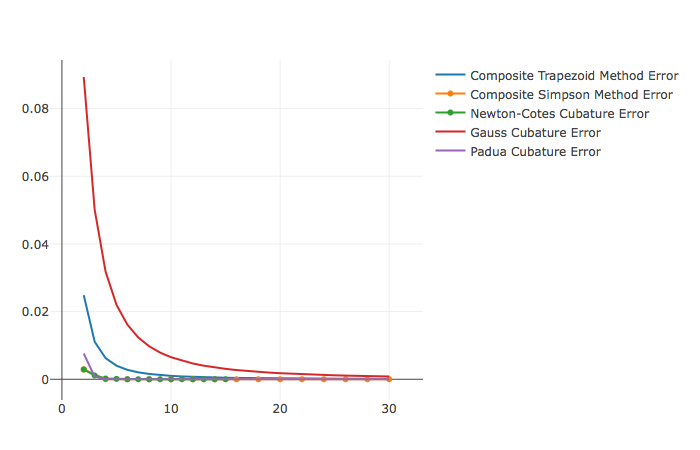
\includegraphics[scale=0.7]{mainfun.png}
\captionof{figure}{Wykres błędu względnego w zależności od n.}
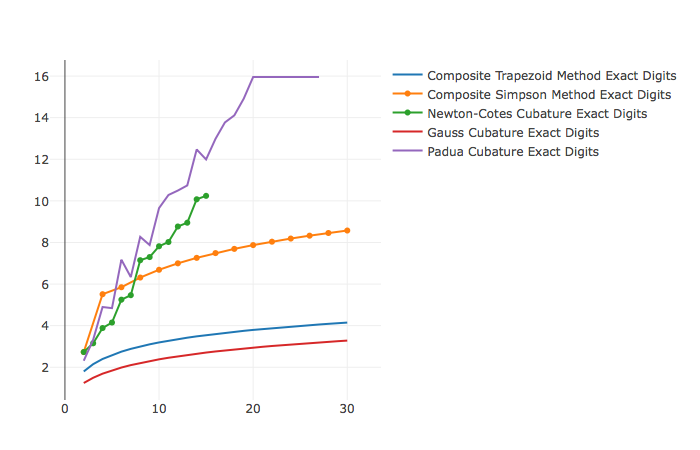
\includegraphics[scale=0.7]{mainfund.png}
\captionof{figure}{Wykres liczby cyfr dokładnych wyniku kubatury w zależności od n.}
Od razu możemy zauważyć bardzo dużą dokładność osiąganą przez kubaturę w punktach Padewskich, zadziwiająco dużą dokładność kubatur Newtona-Cotesa oraz bardzo słabą dokładność kubatury Gaussa-Czebyszewa.

\subsection{Funkcja Franke'go (b).}
Funkcja Franke'go jest często wykorzystywaną funkcją dla sprawdzenia dokładności interpolacji czy całkowania w dwóch wymiarach. \\
\begin{center}
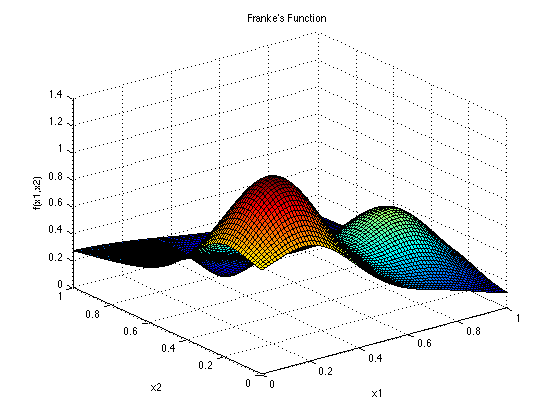
\includegraphics[scale=0.5]{franke2d.png}
\captionof{figure}{Wykres funkcji Frankego, źródło: \emph{https://www.sfu.ca/\textasciitilde ssurjano/franke2d.html}}
\end{center}
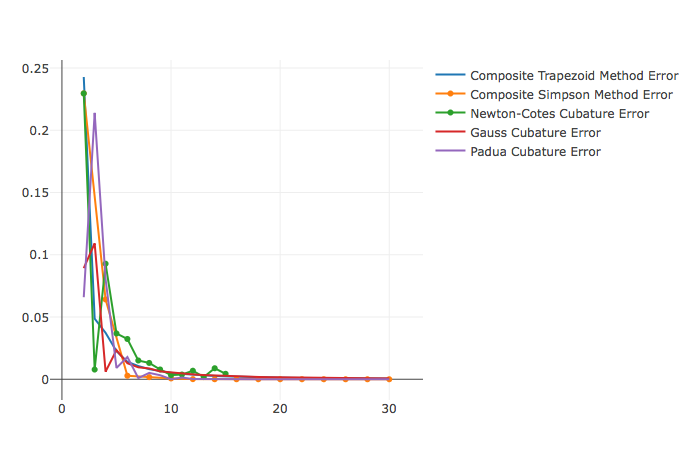
\includegraphics[scale=0.7]{franke.png}
\captionof{figure}{Wykres błędu względnego w zależności od n.}
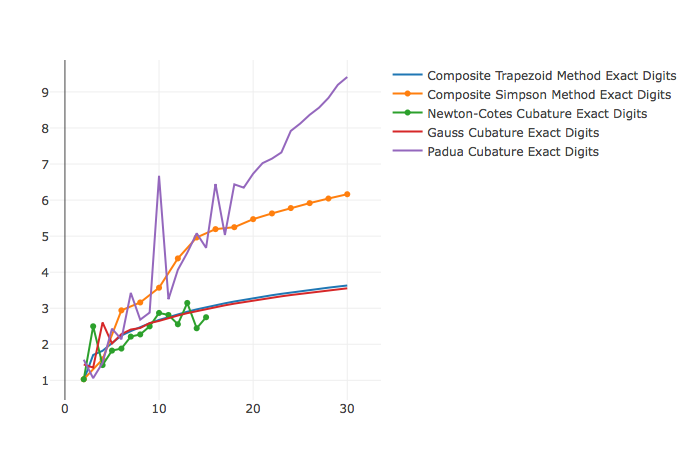
\includegraphics[scale=0.7]{franked.png}
\captionof{figure}{Wykres liczby cyfr dokładnych wyniku kubatury w zależności od n.}
Możemy zauważyć, że dokładność kubatury Newtona-Cotesa się psuje, a kubatura w punktach Padewskich znowu zachowuje się najlepiej.
Możemy też zauważyć, że złożony wzór Simpsona jest bardzo dokładny. Prawdopodobnie ze względu na budowę funkcji f, tj. trzech kopuł funkcji \(e^{-ax^2 - by^2}\), które są dobrze przybliżane przez parabole.


\subsection{Funkcje (c) oraz (d).}
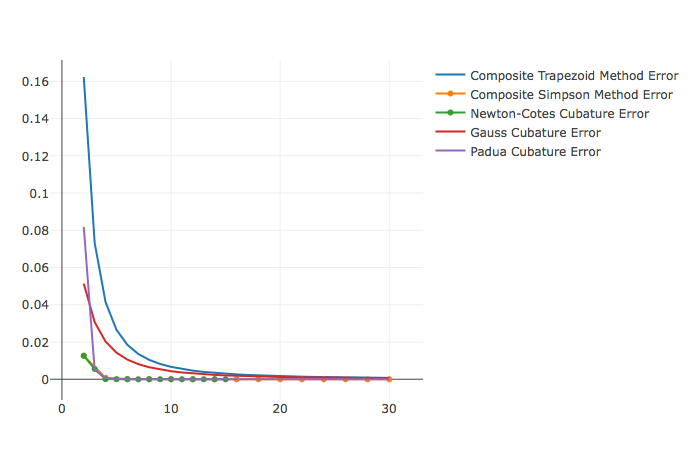
\includegraphics[scale=0.7]{sin.png}
\captionof{figure}{Wykres błędu względnego w zależności od n dla funkcji (c).}
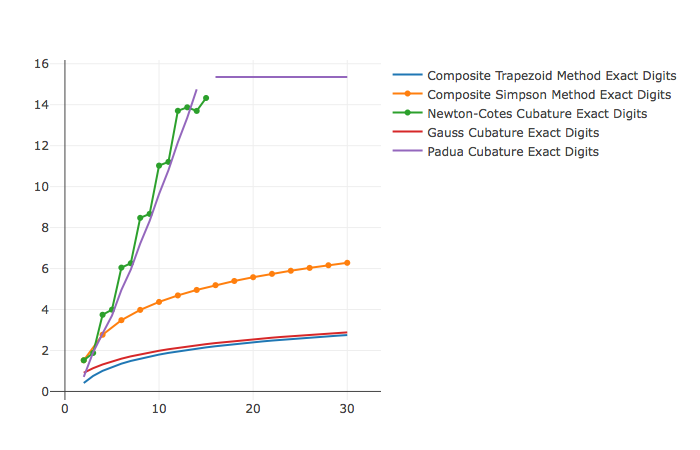
\includegraphics[scale=0.7]{sind.png}
\captionof{figure}{Wykres liczby cyfr dokładnych wyniku kubatury w zależności od n dla funkcji (c).}
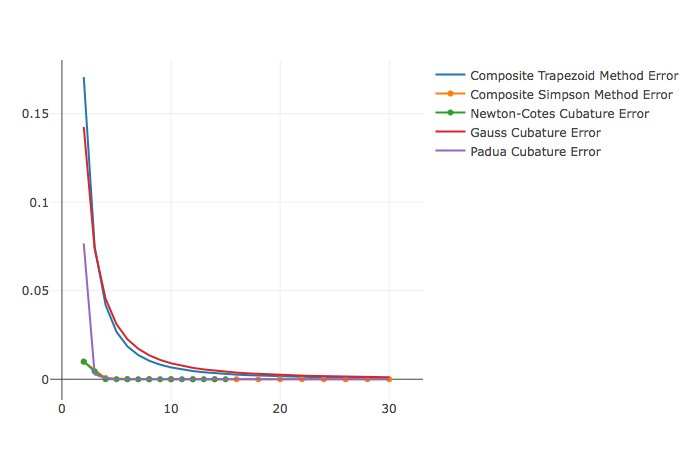
\includegraphics[scale=0.7]{exp.png}
\captionof{figure}{Wykres błędu względnego w zależności od n dla funkcji (d).}
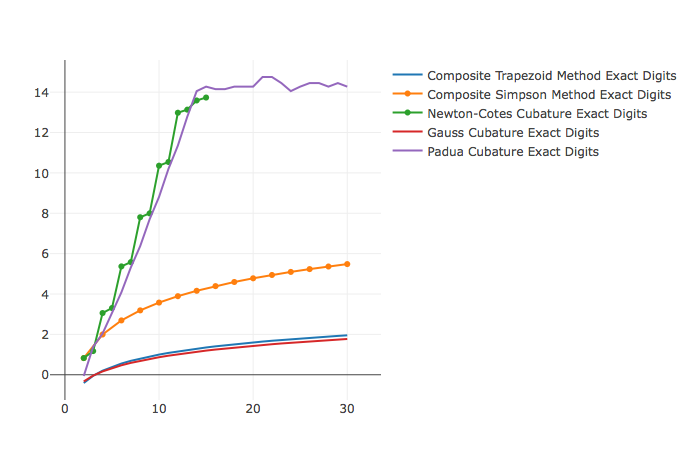
\includegraphics[scale=0.7]{expd.png}
\captionof{figure}{Wykres liczby cyfr dokładnych wyniku kubatury w zależności od n dla funkcji (d).}
W obu przypadkach, kubatura w punktach Padewskich oraz kubatura Newtona-Cotesa wykazują największą dokładność.
Oprócz tego możemy zauważyć, że dokładność kubatury Gaussa jest zbliżona do dokładności złożonego wzoru trapezów niemal we wszystkich przypadkach.
\subsection{Funkcja (e).}
Żeby \emph{obronić} kubaturę Gaussa wykonajmy test dla funkcji (e). \\
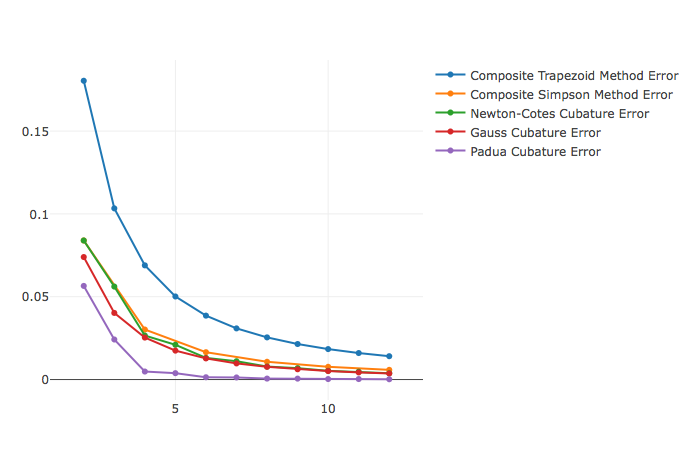
\includegraphics[scale=0.7]{sqrt.png}
\captionof{figure}{Wykres błędu względnego w zależności od n dla funkcji (e).}
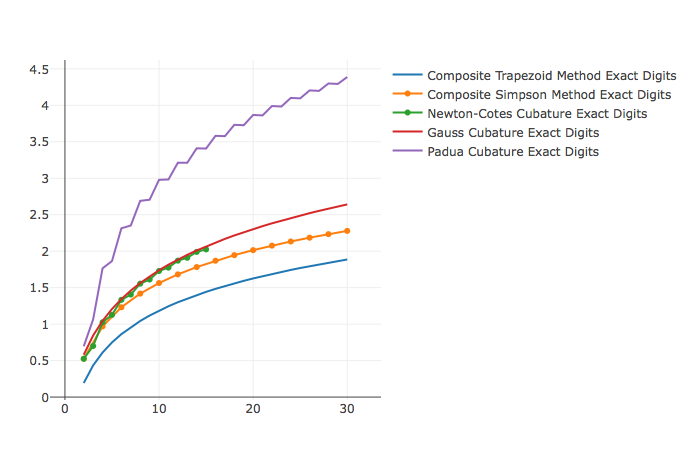
\includegraphics[scale=0.7]{sqrtd.png}
\captionof{figure}{Wykres liczby cyfr dokładnych wyniku kubatury w zależności od n dla funkcji (e).}
Tutaj zbieżność kubatury Gaussa jest zdecydowanie lepsza.
Weźmy też pod uwagę, że kubatura Gaussa-Czebyszewa w odpowiednio wielu punktach da dokładne wyniki dla całek postaci \( \int_{-1}^{1} \int_{-1}^{1} \frac{x^ay^b}{\sqrt{1-x^2}\sqrt{1-y^2}} dydx \).

\subsection{Efekt Rungego dla \(\frac{1}{1 + 25x^2 + 25y^2}\).}
Chcemy także zbadać, czy efekt Rungego występuje także w przypadku kubatur Newtona-Cotesa.
Analogicznie do przypadku jednowymiarowego, będziemy chcieli przybliżyć całkę
\begin{equation*}
  \int_{-1}^{1} \int_{-1}^{1}\frac{1}{1 + 25x^2 + 25y^2} dydx = 0.43619341081228\dots
  \end{equation*}
kolejnymi \(C_{n,n}^{NC}(f)\).\\
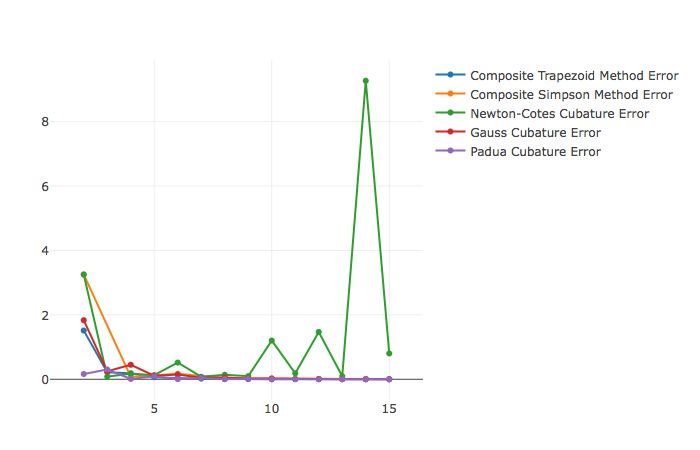
\includegraphics[scale=0.7]{runge.png}
\captionof{figure}{Wykres błędu względnego w zależności od n dla funkcji Rungego.}
Możemy zauważyć, że dla parzystych wartości \(n\) (czyli przy interpolacji w \((n+1)^2\)),
 wartość kubatury zaczyna znacząco odbiegać od wartości całki.
 Dla nieparzystych \(n\)-ów to zjawisko również zachodzi, jednak błąd nie jest aż tak duży jak dla chociażby \(n \in \{ 10, 12, 14\} \) - możemy zobaczyć, że dla \(n = 15\) wartość kubatury również jest obarczona dużym błędem

\subsection{Wnioski z testów numerycznych.}
Biorąc pod uwagę wyniki testów numerycznych, możemy zauważyć, że zdecydowanie najlepiej w ogólnym przypadku zachowuje się kubatura w punktach Padewskich.
Ważną obserwacją jest także fakt, że wszystkie te kubatury, poza powyższą, wykorzystują \((n+1)^2\) punktów,
a kubatura w punktach Padewskich wykorzystuje \(\frac{(n+1)(n+2)}{2}\) punktów, czyli około połowę mniej.
Oprócz tego wagi tej kubatury możemy także obliczyć niezależnie od funkcji i przechowywać, bez potrzeby liczenia ich w trakcie wykonywania programu.
Niemniej jednak możemy zauważyć, że we wszystkich przypadkach rząd kwadratury rośnie zdecydowanie wolniej względem liczby punktów, które wykorzystujemy, niż w przypadku jednowymiarowym.
Innymi słowy, żeby dostać kubaturę o rzędzie o jeden bądź dwa wyższym, musimy dołożyć nie jeden punkt, a około \(2n+1\) punktów (bądź w przypadku kubatury w punktach Padewskich około \(n+2\)) punktów).
Oczywiście problem całkowania dla wyższych wymiarów prawdopodobnie cierpi na tym jeszcze bardziej, bowiem w przypadku funkcji trzech zmiennych możemy przewidywać, że musimy dokładać około \(O(n^2)\) punktów, czterech zmiennych - \(O(n^3)\), etc.

\section{Metoda Monte Carlo.}
Okazuje się, że dość powszechnie używaną metodą jest metoda Monte Carlo.
Jest bardzo prosta do zrozumienia, jak i do zaimplementowania.
Przypomnimy ideę stojącą za tą metodą: Gdy dla wszystkich \((x,y) \in [a,b]\times[c,d]\) zachodzi \(f(x,y) \geq 0 \) to zamknijmy funkcję \(f(x,y)\) w prostopadłościanie o podstawie \([a,b] \times [c,d]\) - nazwijmy go \(P\). Losujemy określoną liczbę punktów \((x,y,z) \in P\) ,
a niech zbiór \(A\) będzie zbiorem tych punktów. Dla każdego z nich sprawdzamy, czy \(f(x,y) \leq z\).
Wtedy \begin{equation}
  \int_a^b \int_c^d f(x,y) dy dx \approx \frac{|\{(x,y,z): (x,y,z) \in A \wedge f(x,y) \leq z\}|}{|A|}(b-a)(d-c)\Bigg(\sup_{x,y \in [a,b]\times [c,d]} f(x,y)\Bigg)
\end{equation}
Jeśli chcemy rozpatrywać funkcję \(f\), która może być ujemna na tym przedziale, to możemy rozbić powyższą całkę na dwie osobne dla funkcji \(max(f,0)\) oraz \(min(f,0)\) i odjąć je od siebie, bądź przesunąć funkcję o wartość \(\inf_{x,y \in [a,b]\times [c,d]} f(x,y)\) do góry i odjąć objętość dodanego prostopadłościanu.
Oczywiście mamy do czynienia z metodą, która opiera się na losowaniu punktów, przez co istnieje prawdopodobieństwo, że wartość naszej całki będzie obarczona bardzo dużym błędem.
Jednak jeśli nie zależy nam aż tak na precyzyjnym wyniku, a na tym by procedura działała szybko, bądź mierzymy się ze specyficznymi obszarami całkowania, to metoda Monte Carlo jest jedną z lepszych i bardziej efektywnych metod.
Istnieją pewne metody wyprowadzone z metody Monte Carlo, o których możemy przeczytać w \cite{JDFKIS}.
\section{Podsumowanie.}
Pomimo problemów dotyczących wielomianów ortogonalnych, widzimy, że możemy łatwo rozszerzać kwadratury interpolacyjne na kubatury. Jednak jednocześnie, wzrasta nam liczba punktów w których interpolujemy naszą funkcję.
Możemy zauważyć, że w celu otrzymania w miarę dokładnej kubatury (tj. rzędu wyższego niż \(n\)) potrzebujemy co najmniej \(\frac{(n+1)(n+2)}{2}\) punktów i to w przypadku optymalnej kwadratury w punktach padewskich (wtedy mamy kwadraturę rzędu \(2n-1\)).
Znacznie częściej wykorzystujemy około \(n^2\) punktów. Warto też zauważyć, że rozważaliśmy dość szczególny przypadek całki podwójnej, gdzie obszarem całkowania był prostokąt.
W ogólnym przypadku, czyli dla dowolnego obszaru całkowania, ciężko jest znaleźć bardziej efektywną metodę niż metoda Monte Carlo.
\begin{thebibliography}{9}
\itemsep10pt
\bibitem{JMJ} J. i M. Jankowscy, \emph{Przegląd metod i algorytmów numerycznych}, cz. 1, WNT, 1981.
\bibitem{AR} A. Ralston, \emph{A First Course in Numerical Analysis}, Dover Publications, 1965.
\bibitem{CK} W. Cheney, D. Kincaid, \emph{Analiza numeryczna}, WNT, 2006.
\bibitem{IK} E. Isaacson, H. B. Keller, \emph{Analysis of Numerical Methods}, Dover Publications, 1966.
\bibitem{PS} P. K. Suetin, \emph{Orthogonal Polynomials in Two Variables}, Gordon and Breach Science Publishers, 1999.
\bibitem{YX} Y. Xu, \emph{Orthogonal Polynomials Of Several Variables}, arXiv:1701.02709, 2017.
\bibitem{PO} P. Olver, \emph{On Multivariate Interpolation}, 2005.
\bibitem{BMVX} L. Bos, S. De Marchi, M. Vianello, Y. Xu, \emph{Bivariate Lagrange Interpolation At The Padua Points: The Ideal Theory Approach}, 2007
\bibitem{YX2} Y. Xu, \emph{Optimal points for Cubature Rules and Polynomial Interpolation on a Square}, arXiv:1709.00651, 2017.
\bibitem{CMSV} M. Caliari, S. De Marchi, A. Sommariva, M. Vianello, \emph{Padua2DM: fast interpolation and cubature at the Padua points in Matlab/Octave}, 2010.
\bibitem{JDFKIS} J. Dick, F. Y. Kuo, I. H. Sloan, \emph{High-dimensional integration: The quasi-Monte Carlo way}, Cambridge University Press, 2013.
\end{thebibliography}
\end{document}
